\documentclass[12pt]{article}

\usepackage[]{amsmath}
\usepackage[]{amsthm}
\usepackage[]{amsfonts}
\usepackage[]{amssymb}
\usepackage{blindtext}
\usepackage[a4paper, total={6in, 8in}]{geometry}
\usepackage{graphicx}
\graphicspath{{/home/dimitri/Pictures}}

\usepackage{listings}
\usepackage{color}

\definecolor{dkgreen}{rgb}{0,0.6,0}
\definecolor{gray}{rgb}{0.5,0.5,0.5}
\definecolor{mauve}{rgb}{0.58,0,0.82}

\lstset{frame=tb,
  language=Java,
  aboveskip=3mm,
  belowskip=3mm,
  showstringspaces=false,
  columns=flexible,
  basicstyle={\small\ttfamily},
  numbers=left,
  numberstyle=\small\color{black},
  keywordstyle=\color{blue},
  commentstyle=\color{dkgreen},
  stringstyle=\color{mauve},
  breaklines=true,
  breakatwhitespace=true,
  tabsize=3
}

\title{EECS3101 Assignment 2}

\author{Jerry Wu (217545898)}

\date{Due Feb. 17 2023 at 22:00}

\begin{document}
\maketitle

\subsection*{Question 1}

\begin{itemize}
    \item[a)] Upon inspection, we can see that the worst case happens in the first if statement, where the loop has to run 500 times. We know that the sample space for the number of times "cha-ching" is printed is the following:: $\Omega=\{0,5,20,500\}$. Printing it 500 times would take more time than printing it 0, 5 or 20 times, so we can safely say that it is the worst case.
    
    \item[b)] Our job is to calculate $P(X=500)$ where $X$ is a discrete random variable signifying the number of times "cha-ching" is printed. We know that $A$, $B$, and $C$ are each independent of one another, and they each have a $\frac{1}{m}$ chance of taking on the value of 1. Because of independence, we can multiply each probability together, thus we have that $P(X=500)=\frac{1}{m^3}$.
    \item[c)] The best case (from an algorithm analysis standpoint, not to the player's benefit) would be when the program prints it 0 times. It prints out 0 times if none of the if statement conditions are matched, and 0 is the smallest number in the sample space, so we can say that it is the best case.
    \item[d)] We know that the probability for any 2 of the reels to be equal is $\frac{1}{m}$. In the best case, none of the reels are equal, whereby we can take the complement of the probability $P(X=0)=1-\frac{1}{m}=\frac{m-1}{m}$.
    \item[e)] We need all probabilities for each case in $\Omega$ to do this problem. We have the probability mass function for $X$::
    

    $P(X=x)=\begin{cases}
        \frac{1}{m^3} & x=500 \\
        \frac{1}{m^2} & x=20 \\
        \frac{1}{m} &x=5\\
        \frac{m-1}{m} & x=0 
    \end{cases}$

    To find the expected return value, we just need to calculate the negative $E(X)$. To do this, we can use the formula::
    \begin{align*}
        E(X)=-\sum_{x\in\Omega}(x-2)P(X=x)=2P(X=0)-3P(X=5)-18P(X=20)-498P(X=500)
    \end{align*}

    The reason we subtract $x$ by 2 is because we subtract money by 2 each time the slot machine is run.

    \begin{align*}
        =2\left(\frac{m-1}{m}\right)-3\left(\frac{1}{m}\right)-18\left(\frac{1}{m^2}\right)-498\left(\frac{1}{m^3}\right)
    \end{align*}
    
    After some simplification we have that::

    \begin{align*}
        E(X)=\frac{2m-5}{m}-\frac{18}{m^2}-\frac{498}{m^3}
    \end{align*}


    \item[f)] We can do this by trial and error. The result I got was $m=10$, since the expression returns a value of 0.82 which is between 0.8 and 1.
\end{itemize}

\subsection*{Question 2}

\begin{itemize}
    \item[a)] The first 3 layers of the recursion tree is attached below::\\
    
    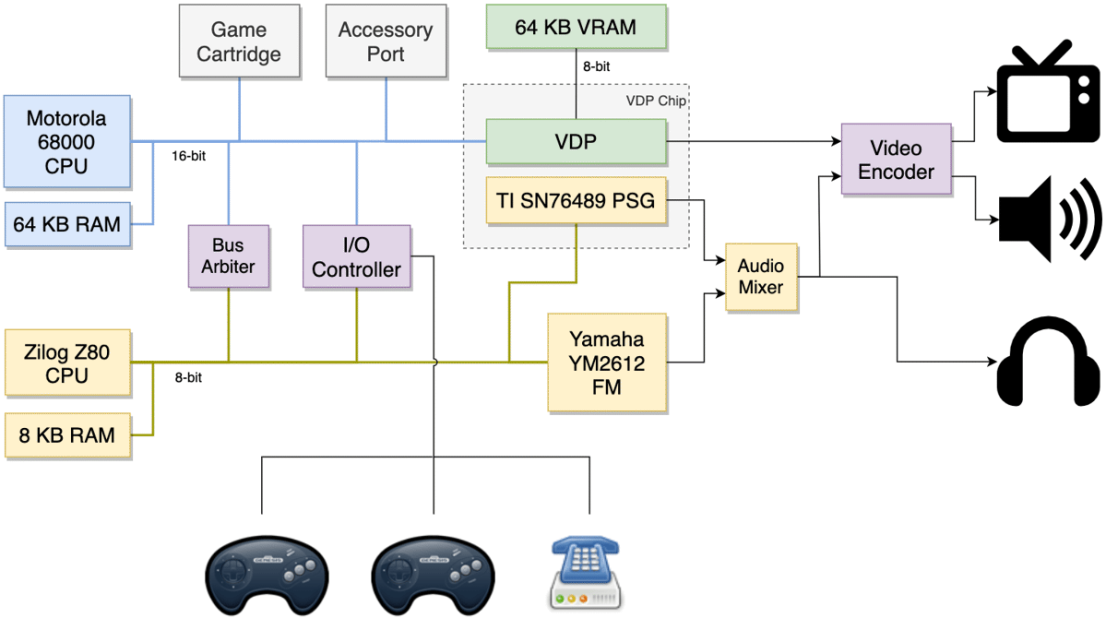
\includegraphics[scale=0.35]{diagram}

    Here we can see that there are $n$ levels in the tree and the number of nodes in each level will double each time we move down a level. From here, if we count the nodes, it is clear that there are $2^n$ many nodes in the tree. Anything that is exponentially increasing for runtime is unacceptably slow. This is due to redundant recursive calls.

    \item[b)] To reduce the complexity of this algorithm, we can use a dynamic programming solution (bottom up approach).
    \begin{lstlisting}
//pre: n>=1
//post: return S_n

int GetS(int n)
{
    int ans[] = array of size n+1;
    ans[0] = 1;
    ans[1] = 2;
    for(int i = 2, i <= n; i++)
    {
        ans[i] = 2*ans[i-1] + 3*ans[i-2]
    }

    return ans[n];
}
    \end{lstlisting}

    This reduces the problem's complexity down to $\Theta(n)$ because we \textbf{iterate through an array} $n-1$ times. This yields the same output as the recursive version because we have the same base cases in the first two indices of the array upon initialization.

    \item[c)] Unfortunately after many hours of suffering, blood, sweat, and tears, I was unable to devise a solution to make the runtime complexity to be $\Theta(\log(n))$, however, I did improve it from $\Theta (2^n)$ to $\Theta (n)$, which is a significant improvement.
\end{itemize}

\end{document}